
\section{WaveMix Model}

Natural images possess several important statistical properties. First, they are inherently structured, exhibiting strong regularities and correlations at multiple scales \cite{field1993scale,ruderman1994statistics,lee1996image,parraga2002spatiochromatic,zoran2009scale}. These properties stem from the physical processes involved in image formation, such as the interaction of light with surfaces and the geometry of the scene. One key characteristic of natural images is the presence of self-similarity and scale invariance \cite{field1993scale,zoran2009scale}. That is, similar patterns and structures appear at different scales, making natural images well-suited for multi-resolution analysis using wavelets.

Wavelets have been widely used in image processing tasks due to their ability to represent images at multiple scales and orientations \cite{ruikar2010image,guo2017deep,mahmood2018facial}. For instance, wavelet-based techniques have been employed for image compression \cite{lewis1992image}, feature extraction \cite{mowlaei2002feature}, and medical image analysis \cite{ranaware2016detection,nayak2016brain}. The success of wavelets in these applications can be attributed to their ability to efficiently capture both spatial and frequency information, making them ideal for analyzing the complex structures present in natural images.

Recent advances in deep learning have further highlighted the relevance of wavelet-based representations. Scattering networks, which use predefined wavelet filters followed by non-linear operations, have been shown to achieve impressive performance on various image classification tasks \cite{bruna2013invariant}. These networks leverage the multi-scale and multi-orientation properties of wavelets to extract stable and discriminative features. More recently, researchers have explored integrating wavelet transforms into convolutional neural networks (CNNs) to improve their robustness and performance \cite{li2020wavelet,liu2018multi,kumar2017cnn,williams2018wavelet}. For example, Wavelet Integrated CNNs (WaveICNNs) have been proposed for noise-robust image classification \cite{li2020wavelet}, and wavelet pooling techniques have been developed to preserve important image details while reducing spatial resolution \cite{williams2018wavelet}.

Moreover, wavelet-based methods have shown promise in image segmentation tasks, where precise localization of boundaries is crucial. The WaveSNet architecture integrates wavelet transforms into a deep network to enhance segmentation accuracy by leveraging both global context and local details \cite{li2020wavesnet}. These approaches demonstrate the continued relevance of wavelet theory in modern computer vision applications, particularly in scenarios where capturing the hierarchical structure of natural images is essential.

The proposed framework's main concept is to stack \( N \) WaveMix blocks, which are fully convolutional in both spatial dimensions, ensuring that the spatial resolution of the feature maps remains consistent across the blocks. While some CNNs are fully convolutional, vision transformer models typically preserve the sequence length (a flattened version of spatial resolution). By combining these two approaches, the WaveMix architecture becomes highly flexible, capable of adapting to different image sizes and tasks. For example, pixel maps for semantic segmentation or image enhancement can be directly produced with this framework \cite{jeevan2024wavemix}. 

Additionally, by adding an optional MLP layer for channel mixing, followed by global average pooling and softmax, the model can be adapted for image classification across a variety of image sizes. Unlike transformer models, which process images as sequences of patches, WaveMix treats the image as a 2D grid. To further enhance flexibility, the input image \( x' \in \mathbb{R}^{H \times W \times 3} \) is first passed through a convolutional layer to increase the channel count to the embedding dimension \( C \) (i.e., \( x \in \mathbb{R}^{H \times W \times C} \), where \( C \) is a hyperparameter) \cite{jeevan2024wavemix}.

\subsection{WaveMix}

\begin{figure}
    \centering
    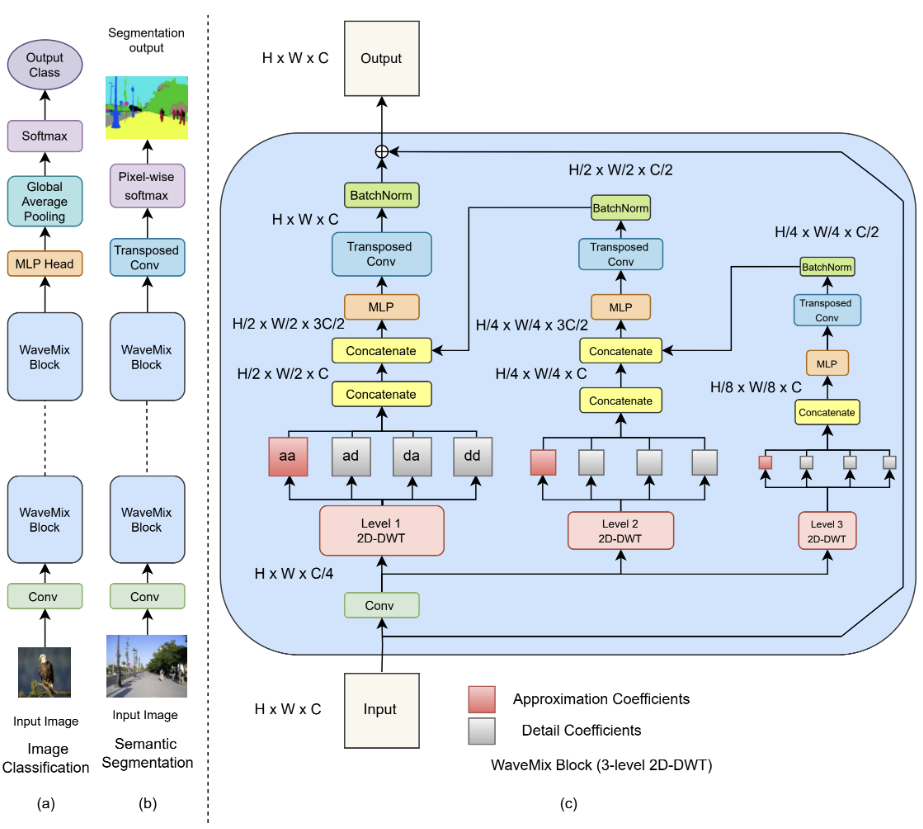
\includegraphics[width=0.8\linewidth]{related-work/image/wavemix_architecture.png}
    \caption{WaveMix architecture for (a) image classification (b) semantic segmentation, along with (c) details of the WaveMix block \cite{jeevan2024wavemix}}
    \label{fig:wavemix_arch}
\end{figure}


The WaveMix block applies a series of transformations to extract and process image features efficiently\cite{jeevan2024wavemix}:

\textbf{Initial Feature Extraction using Convolution}

The input image tensor \( x_{\text{in}} \) undergoes a convolution operation using learnable parameters \( \xi \). This convolution extracts spatial features and reduces the embedding dimension \( C \) by a factor of 4 to compensate for the channel expansion in later steps. This step ensures that only relevant feature maps are used for wavelet decomposition. The operation is represented by the following equation:

\[
x_0 = c(x_{\text{in}}, \xi)
\]

\textbf{Multi-level 2D Wavelet Transform (2D-DWT)}

The Discrete Wavelet Transform (DWT) decomposes \( x_0 \) into four sub-bands per level \( l \). These sub-bands represent the approximation and details of the image at multiple scales. The sub-bands include:
\begin{itemize}
    \item \( w^l_{aa}(x_0) \): Approximation (low-frequency components)
    \item \( w^l_{ad}(x_0) \): Horizontal details
    \item \( w^l_{da}(x_0) \): Vertical details
    \item \( w^l_{dd}(x_0) \): Diagonal details
\end{itemize}
The spatial resolution is halved at each level, but the number of channels increases fourfold due to the concatenation of these sub-bands. This process captures both scale-invariant (low-frequency) and edge-like (high-frequency) features. The equation for this step is:

\[
x_l = \left[w^l_{aa}(x_0) \oplus w^l_{ad}(x_0) \oplus w^l_{da}(x_0) \oplus w^l_{dd}(x_0) \right]
\]

Unlike traditional CNN pooling, the 2D-DWT preserves information while reducing spatial dimensions, making it an effective feature extraction method.

\textbf{Feature Aggregation Across Levels}

Features from level \( l \), denoted as \( x_l \), are concatenated with the higher-level feature map \( \hat{x}_{l+1} \). This aggregation allows information from deeper layers, which have a larger receptive field, to propagate to shallower layers. The concatenation ensures long-range spatial interactions and enables the efficient learning of hierarchical features. This process is represented by the following equation:

\[
\hat{x}_l = [x_l \oplus \hat{x}_{l+1}], \quad l \in \{1, ..., L-1\}
\]

\textbf{Channel Mixing using MLP (1×1 Convolution)}

The feature maps undergo channel mixing using a Multi-layer Perceptron (MLP) layer and 1×1 convolutions. The MLP applies two 1×1 convolutions with a GELU non-linearity in between, expanding the channels temporarily to improve feature extraction. A transposed convolution is then used to double the spatial resolution while halving the number of channels to restore balance. Additionally, batch normalization is applied to stabilize training and prevent exploding gradients. This step is represented by the following equation:

\[
\hat{x}_l = b(t(m(\hat{x}_l, \theta_l), \phi_l), \gamma_l); \quad \forall l > 1
\]

\textbf{Residual Connection for Stable Training}

The final output of the WaveMix block is obtained by adding the processed feature map \( \hat{x}_1 \) to the original input \( x_{\text{in}} \). This residual connection helps ease the flow of gradients during backpropagation, reducing vanishing gradients and stabilizing training. The equation for this step is:

\[
x_{\text{out}} = \hat{x}_1 + x_{\text{in}}
\]


The key takeaways from this approach include: Convolution Before DWT, which ensures that only trained and relevant feature maps are used for wavelet decomposition; 2D-DWT for Multi-scale Feature Extraction, which reduces spatial dimensions while increasing channels and captures both global (low-frequency) and local (high-frequency) features; Feature Aggregation Across Levels, which allows information to flow from deeper levels to shallower ones; MLP (1×1 Convolution) for Channel Mixing, which enhances feature interactions across channels; Transposed Convolution for Spatial Resolution Recovery, which upsamples feature maps while maintaining efficiency; and Residual Connection for Stability, which helps with efficient gradient flow during training. 

\subsection{WaveMix-Lite}

\begin{figure}
    \centering
    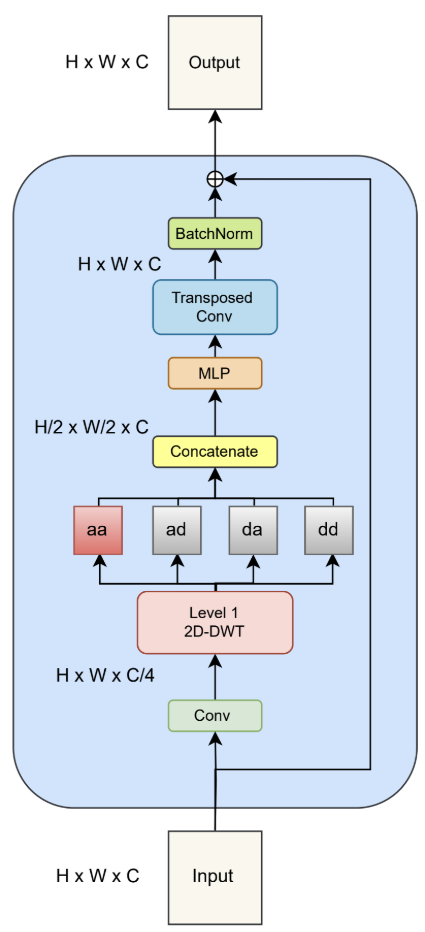
\includegraphics[width=0.3\linewidth]{related-work/image/wavemix_lite_arch.png}
    \caption{A Wavemix-Lite Block \cite{jeevan2024wavemix}}
    \label{fig:wavemix_lite_arch}
\end{figure}

A more lightweight and computationally efficient version of the WaveMix block is also introduced, referred to as \textbf{WaveMix-Lite}. This variant is specifically designed to accommodate models with larger embedding dimensions while remaining within the memory constraints of a single 16 GB GPU.

The input to WaveMix-Lite is first passed through a convolutional layer that reduces the embedding dimension by a factor of four. This reduction ensures that the output of the subsequent 2D Discrete Wavelet Transform (DWT), once concatenated, matches the original input dimension. To further reduce computational overhead and the number of parameters, WaveMix-Lite employs only a single-level 2D DWT.

This architecture is primarily utilized in scenarios where high embedding dimensions are required. The increased dimensionality allows the model to effectively capture long-range global dependencies within a single-level 2D DWT, thereby removing the necessity for multiple DWT levels. Consequently, we replace the standard WaveMix block with WaveMix-Lite in models where the embedding dimension exceeds 64.

\subsection{WaveMixSR}

\begin{figure}
    \centering
    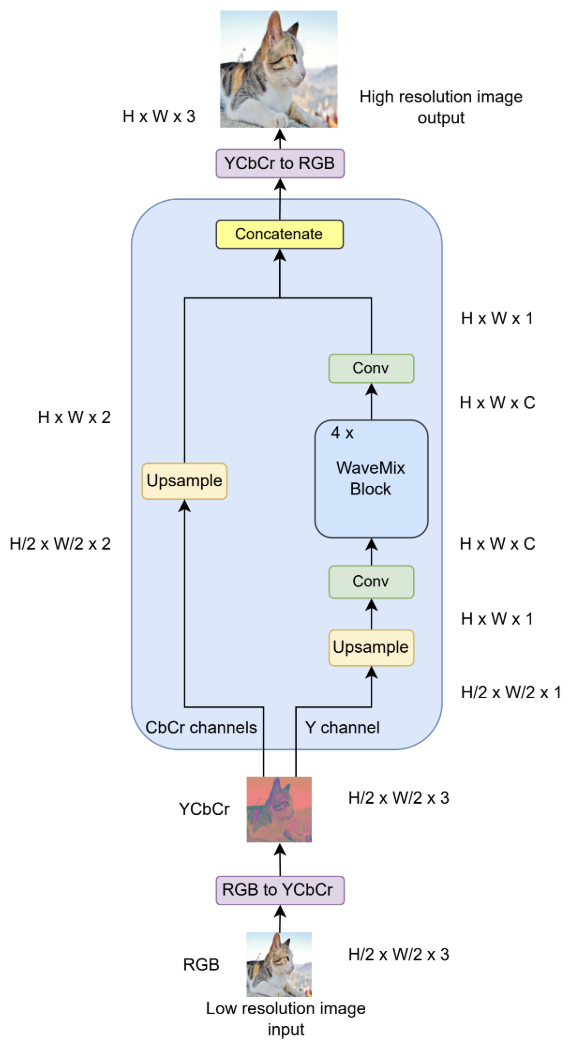
\includegraphics[width=0.3\linewidth]{related-work/image/wavemix_sr_architecture.png}
    \caption{Architecture of WaveMixSR along with the details of the WaveMix block. Architecture is shown for 2× super-resolution. For 3× and 4× super-resolution, only the upsample blocks are modified, while the other blocks intact are kept \cite{jeevan2024wavemix}.}
    \label{fig:wavemix_sr_arch}
\end{figure}

The low-resolution (LR) input image in RGB space is converted to YCbCr space before being sent to the model. The YCbCr color space separates the image into three channels: Y (luma), Cb (blue-difference chroma), and Cr (red-difference chroma). The Y channel represents the luminance information of the image, while the Cb and Cr channels represent the chrominance information.

WaveMixSR has two paths—one for handling the Y channel and another for the CbCr channels of the input image. Typically, in super-resolution (SR) techniques, only the Y channel is used for the path with parametric learning because it contains most of the image details and is less affected by color changes. This approach has been shown to improve the performance of deep learning-based SR methods \cite{dong2015image}. The same idea is followed in WaveMixSR, where only the Y channel is sent through the path with WaveMix blocks to focus on improving the resolution of the LR image while ignoring the color changes.

For $2\times$ SR, the first path takes the Y-channel feature map, $y \in \mathbb{R}^{\frac{H}{2} \times \frac{W}{2} \times 1}$ of the input image and sends it through a parameter-free upsampling layer that resizes the low-resolution Y-channel image to high resolution using bilinear or bicubic interpolation. For $3\times$ and $4\times$ SR, corresponding upsampling blocks that upsample the image to HR are used. The output of the upsampling block, $y \in \mathbb{R}^{H \times W \times 1}$, is sent to a convolutional layer to increase the number of feature maps from 1 to $C$. The output feature maps from the convolutional layer, $x_{\text{in}} \in \mathbb{R}^{H \times W \times C}$, are sent to the WaveMix blocks. Four WaveMix blocks are connected in series in our model to create high-resolution feature maps. The output $x_{\text{out}} \in \mathbb{R}^{H \times W \times C}$ from the final WaveMix block is then passed through a convolutional layer which reduces the channel dimension $C$ and returns a single-channel output $y_{\text{out}} \in \mathbb{R}^{H \times W \times 1}$.

The second parallel path in WaveMixSR takes the two channels of CbCr and simply passes them through an upsampling layer (bilinear/bicubic) to increase the resolution to the final desired output size. This high-resolution CbCr output is concatenated with the Y-channel output $y_{\text{out}}$ from the first path, thereby creating the 3-channel YCbCr output. This output is then converted back to the RGB color space to obtain the final high-resolution output image.


\subsection{Waveface Model}

The WaveFace model is an innovative approach to blind face restoration (BFR) that addresses the limitations of existing diffusion model-based methods, such as slow inference speed and poor preservation of facial identity and details. By operating in the frequency domain using Discrete Wavelet Transform (DWT), WaveFace decomposes images into low-and high-frequency components. The low-frequency component, which captures general facial structure, is restored efficiently using a conditional diffusion model (LCD) that leverages degraded inputs as guidance to preserve identity. Meanwhile, the high-frequency components, containing fine-grained details, are recovered in a single step by a unified U-shaped network (HFR). This dual-module framework achieves a speedup in inference compared to traditional diffusion models.

\begin{figure}[htbp]
    \centering
    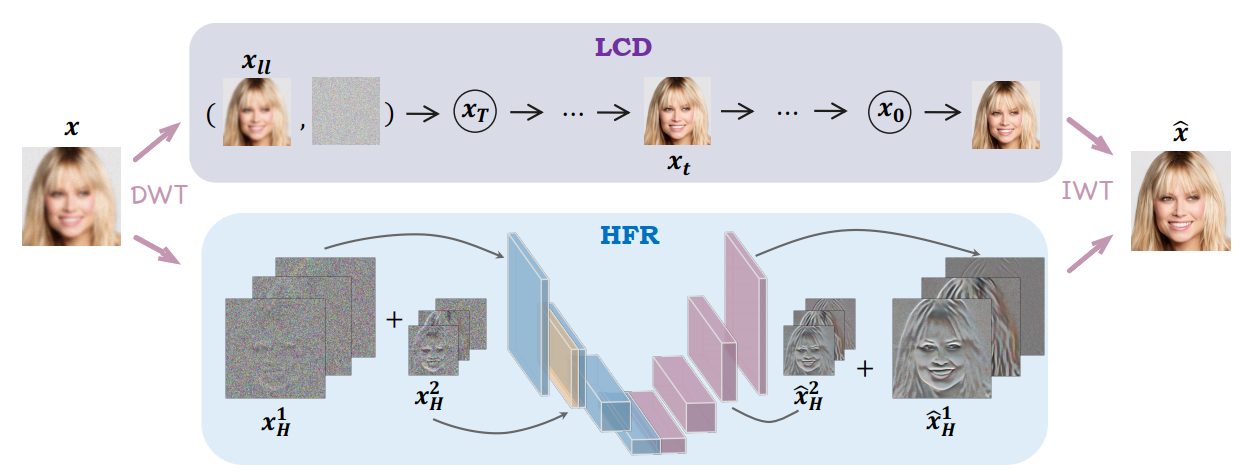
\includegraphics[width=0.8\textwidth]{experiment/images/Waveface_architecture.png}
    \caption{Illustration of Waveface framework}
    \label{fig:waveface_architecture}
\end{figure}

As shown in Figure \ref{fig:waveface_architecture}, WaveFace architecture consists of two distinct stage, LCD and HFR.

In LCD stage, WaveFace model utilize diffusion model (DM) to restore the low-frequency sub-band of high-quality (HQ) images thanks to its powerful generative ability from noisy inputs. However, a fundamental trade-off exists between processing speed and output quality. Diffusion models operating on full-resolution images (512×512+) consume significant computational resources and require lengthy sampling procedures. Although employing deeper wavelet decompositions of low-frequency components improves efficiency, each additional decomposition level sacrifices image details. The central challenge involves determining the ideal DWT decomposition depth that achieves the best compromise between computational performance and restoration accuracy.

In HFR stage, while the LCD module successfully reconstructs the fundamental facial structure, the intricate details that enhance realism predominantly exist in the high-frequency components (Figure~1). These high-frequency sub-bands exhibit varying dimensions across different DWT levels, which would normally require multiple specialized models for complete restoration. To maintain computational efficiency, we employ a unified U-shaped network capable of processing all high-frequency sub-bands simultaneously through a single forward pass.

For an image pair $(\mathbf{x},\mathbf{y})$ with their respective high-frequency components:
\begin{align*}
\mathbf{x}_H^j &= \{\mathbf{x}_{lh}^j, \mathbf{x}_{hl}^j, \mathbf{x}_{hh}^j\} \\
\mathbf{y}_H^j &= \{\mathbf{y}_{lh}^j, \mathbf{y}_{hl}^j, \mathbf{y}_{hh}^j\}
\end{align*}
where $j \in \{1,2\}$ denotes the DWT level, the HFR module operates as:

\begin{align}
\mathbf{F}_H^1, \mathbf{F}_H^2 &= \mathcal{U}_{\phi_u}\left(\mathcal{H}_{\phi_{in}}(\mathbf{x}_H^1), \mathcal{F}_{\phi_f}(\mathbf{x}_H^2)\right) \\
\hat{\mathbf{x}}_H^j &= \mathcal{H}_{\phi_{out}^j}(\mathbf{F}_H^j) + \mathbf{x}_H^j, \quad j \in \{1,2\}
\end{align}

The operators $\mathcal{U}(\cdot)$, $\mathcal{H}(\cdot)$, and $\mathcal{F}(\cdot)$ represent U-shaped network with parameters $\phi_u$, convolutional layers with parameters $\phi_{in}$ and $\phi_{out}^j$ lightweight fusion module with parameters $\phi_f$ respectively. The fusion module employs two consecutive ConvBlocks (3$\times$3 and 1$\times$1 convolutions with ReLU activation) followed by concatenation, ensuring efficient processing while maintaining restoration quality.


\subsection{Non-local Fast Fourier Convolution Model}
\begin{figure}[H]
    \centering
    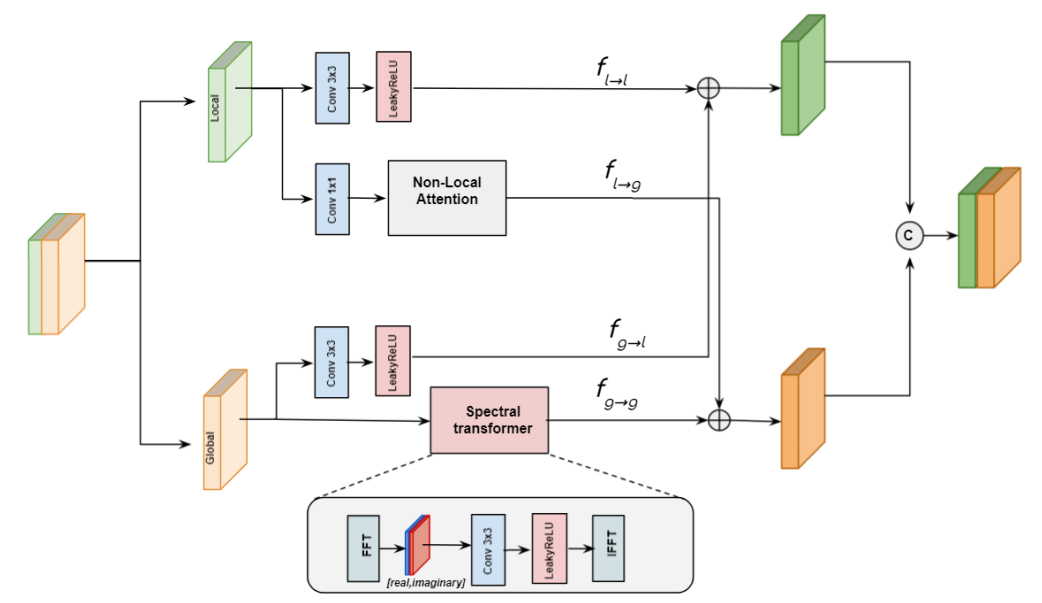
\includegraphics[width=1\linewidth]{experiment/images/NLFCC_architecture.png}
    \caption{Illustration of Non Local-Fast Fourier Convolution (NL-FFC) layer\cite{9857272}.}
    \label{NLFCC_architecture}
\end{figure}

Figure \ref{NLFCC_architecture} illustrates the architecture of the NL-FFC model. In this design, the input features are separated into two categories: local and global features, in the ratio $(1 - \alpha):\alpha$. This separation enables the model to learn four types of feature mappings: local-to-local ($f_{l \rightarrow l}$), local-to-global ($f_{l \rightarrow g}$), global-to-local ($f_{g \rightarrow l}$), and global-to-global ($f_{g \rightarrow g}$):

\begin{align}
f_{l \rightarrow l}(\mathbf{X}^l) &= \text{Conv}_{3 \times 3}^{l \rightarrow l}(\mathbf{X}^l) \\
f_{l \rightarrow g}(\mathbf{X}^l) &= \mathcal{G} \left( \text{Conv}_{1 \times 1}^{l \rightarrow g}(\mathbf{X}^l) \right) \\
f_{g \rightarrow l}(\mathbf{X}^g) &= \text{Conv}_{3 \times 3}^{g \rightarrow l}(\mathbf{X}^g) \\
f_{g \rightarrow g}(\mathbf{X}^g) &= \mathcal{T}(\mathbf{X}^g) \\
\mathbf{Y}^l &= f_{l \rightarrow l}(\mathbf{X}^l) + f_{g \rightarrow l}(\mathbf{X}^g) \\
\mathbf{Y}^g &= f_{l \rightarrow g}(\mathbf{X}^l) + f_{g \rightarrow g}(\mathbf{X}^g)
\end{align}

Local features, which do not require long-range dependencies, are updated using a standard $3 \times 3$ convolution. For the local-to-global mapping, a non-local attention mechanism~\cite{nonlocal} is employed to capture global dependencies based on each pixel's context. Global-to-local transformation is carried out using a $3 \times 3$ convolutional kernel, which estimates each pixel's local feature from its neighborhood.

Global-to-global transformation first converts the features into the frequency domain using a spectral transformation. This increases the receptive field and allows the model to generate enhanced global features. These are then mapped back to the spatial domain. Basically, it leverages Fast Fourier Convolution (FFC) for efficient and wide-context feature extraction. This design choice is grounded in two fundamental properties of the Fourier Transform:

\textbf{Convolution Theorem: Spatial Convolution $\leftrightarrow$ Frequency Multiplication}

One of the foundational principles in signal processing is the Convolution Theorem. It states that convolution in the spatial domain is equivalent to element-wise multiplication in the frequency domain, and vice versa.

Let $x(t)$ and $h(t)$ be two functions. Their convolution in the spatial (or time) domain is defined as:

\begin{equation}
(x * h)(t) = \int_{-\infty}^{\infty} x(\tau) h(t - \tau) \, d\tau
\end{equation}

Applying the Fourier Transform to both sides:

\begin{equation}
\mathcal{F}\{x * h\} = \mathcal{F}\{x\} \cdot \mathcal{F}\{h\}
\end{equation}

In 2D image processing, the same applies:

\begin{equation}
\mathcal{F}\{I * K\} = \mathcal{F}\{I\} \cdot \mathcal{F}\{K\}
\end{equation}

Where:
\begin{itemize}
    \item $I$ is the input image (or feature map),
    \item $K$ is the convolution kernel,
    \item $*$ denotes convolution,
    \item $\cdot$ denotes point-wise multiplication,
    \item $\mathcal{F}$ denotes the Fourier Transform.
\end{itemize}

Thus, instead of performing convolution directly in the spatial domain, which is computationally expensive for large kernels or global operations, we can transform both the input and the kernel to the frequency domain, perform a simple multiplication, and then apply the inverse Fourier Transform to return to the spatial domain.

\textbf{Computational Efficiency of Fourier Multiplication}

Direct convolution of two $N \times N$ feature maps has a computational complexity of $\mathcal{O}(N^2 \cdot k^2)$, where $k$ is the kernel size. In contrast, the Fast Fourier Transform (FFT) allows the computation of the same operation with significantly lower complexity.

\begin{itemize}
    \item Spatial convolution: $\mathcal{O}(N^2 \cdot k^2)$
    \item FFT-based convolution: $\mathcal{O}(N^2 \log N)$
\end{itemize}

This efficiency gain becomes particularly significant for global operations, where the effective kernel size is large or equivalent to the image size. Using FFT, the model can capture long-range dependencies with far fewer operations.


\begin{equation}
f_{g \rightarrow g}(\mathbf{X}^g) = \mathcal{T}(\mathbf{X}^g)
\end{equation}

Where $\mathcal{T}$ includes:
\begin{enumerate}
    \item Applying the FFT to transform features to the frequency domain,
    \item Performing point-wise multiplication with learnable frequency-domain filters,
    \item Applying the inverse FFT to map the output back to the spatial domain.
\end{enumerate}

This approach not only increases the receptive field efficiently but also accelerates convergence by learning more structured frequency components, particularly beneficial for super-resolution tasks.

An important advantage of using the frequency domain---particularly the Fast Fourier Transform (FFT)---is its ability to infer missing high-frequency components. Since super-resolution is a one-to-many mapping problem, learning in the frequency domain allows faster convergence for low-frequency features. These then act as prior knowledge to infer high-frequency components, reducing the size of the potential solution space.

Here, $\mathcal{G}$ denotes the non-local attention model, and $\mathcal{T}$ represents the spectral transformation applied in the frequency domain.

